\documentclass[12pt]{report}
\usepackage{geometry}
\usepackage{graphicx}
\usepackage{setspace}
\usepackage{titlesec}
\usepackage{fancyhdr}
\RequirePackage{helvet}
\usepackage{graphicx}
\usepackage{forest}
\usepackage{listings}
\usepackage{amsmath}

% Section formatting
\titleformat{\chapter}{\normalfont\large\bfseries}{\makebox[1.5cm][l]{\thechapter}}{0pt}{}
\titlespacing*{\chapter}{0pt}{-16pt plus 2pt minus 2pt}{8pt plus 2pt minus 2pt}

\titleformat{\section}{\normalfont\bfseries}{\makebox[1.5cm][l]{\thesection}}{0pt}{}
\titlespacing*{\section}{0pt}{12pt plus 2pt minus 2pt}{6pt plus 2pt minus 2pt}

\titleformat{\subsection}{\normalfont\bfseries}{\makebox[1.5cm][l]{\thesubsection}}{0pt}{}
\titlespacing{\subsection}{0pt}{12pt plus 2pt minus 2pt}{6pt plus 2pt minus 2pt}

\usepackage[backend=biber,style=numeric,sorting=none]{biblatex}
\addbibresource{references.bib}

% Move hyperref to the end and add configuration
\usepackage[
    hidelinks,
    bookmarks=true,
    bookmarksopen=true,
    bookmarksnumbered=true,
    breaklinks=true,
    colorlinks=true,
    linkcolor=blue,
    urlcolor=blue,
    citecolor=blue,
    hyperfootnotes=true,
    pdftoolbar=true,
    pdfpagemode=UseOutlines
]{hyperref}

% Add this after hyperref to ensure proper linking
\makeatletter
\renewcommand*{\bibsetup}{%
  \interlinepenalty=5000\relax
  \widowpenalty=10000\relax
  \clubpenalty=10000\relax
  \raggedbottom
  \frenchspacing
  \tolerance=2000
  \emergencystretch=2em
  \setlength{\bibhang}{\labelsep}%
}
\makeatother


\begin{document}


% Title Page
\begin{titlepage}
\begin{flushright} 
        
\includegraphics[width=8cm]{kiu.jpg} % 
    \end{flushright}
    \begin{center}
       % \vspace*{2cm}
        \Huge
        \textbf{GoSeek - High Performance Search Engine}
        
        \LARGE
       \textbf{Bachelor's Thesis in Computer Science}
\end{center}
        
\begin{center}
        \textbf{Written by}\\
        Romani Todua
        Student ID number: 42001036235

        \vfill

        Kutaisi International University \\[0.3cm]
        School of Math and Computer Science

        \vfill
    \end{center}
        Supervisor: Ia Mosashvili
        Date of submission: 01/15/2025
    
\end{titlepage}

% Declaration of Integrity
\section*{Declaration of Integrity}
I hereby confirm that I have completed this work without external assistance and without using any sources other than those specified, and that this work has not been submitted in the same or similar form to any other authority. All material that has been quoted or paraphrased is cited as such. \\
I have read and acknowledged the policies proposed by Kutaisi International University for the bachelor's theses, particularly the regulations regarding usage rights.

\vspace{2cm}
Date and Place: 1/15/2025 Kutaisi\\

Student's Signature: R.Todua
\clearpage

% Abstract
\begin{center}
    \chapter*{Abstract} 
    \addcontentsline{toc}{chapter}{Abstract} 
\end{center}
Modern data mangement and search systems hardly yield accurate results while searching due to the their nature to always trade off precision
for monetization purposes. Present solutions such as Google and Bing frequently overlook the needed balance between performance and unbiased 
delivery of results in both text matching and text searching. This thesis discusses a novel framework written in Golang, to defeat these constraints 
by using combinations of algorithms. The system uses statistical term weighting methodologies in conjuction with pattern matching techniques
that guarantee accuracy of the results with no ranking bias.Performance testing on large document collections showed extraordinary efficiency
improvments - parallel sorting mechanisms were 76 times faster compared to traditional methdods mainting minimum resource usage. The pattern
detection showed very high throughput, processing large document sets in less than a second.The research here confirms that using eliminating 
ranking bias and using robust algorithms results in faster and more accurate search system. Although at present It's functionality is limited
to the command line, the architecture has been designed modularly to support further scaling.This work forms a critical contribution 
toward the the creation of open source and efficient content discovery systems. 
\newpage
% Table of Contents

\tableofcontents
\renewcommand{\tableofcontents}{
    {
        \clearpage
        \pdfbookmark[0]{\contentsname}{contents}
        \setlength{\parskip}{0pt}
        \setcounter{tocdepth}{1}
        \default@tableofcontents
        \markboth{\contentsname}{\contentsname}
    }
    \pagebreak%
}


\newpage

\clearpage
\chapter{Introduction}
In an era dominated by information and Big Data, its organization and efficient analysis has become an issue which even large scale search engines such as Google and Bing find their limitations in a form of biases introduced by advertising algorithms and the absence of pattern matching.
This thesis explores the design and implementation of a Golang based CLI (Command Line Interface) tool "Goseek" leveraging techniques such as TF-IDF(Term Frequence-Inverse Document Frequency)\cite{wikipedia_tf_idf} ranking and KMP Pattern Matching\cite{wikipedia_kmp} \\
The purpose of search engines are to accurately and efficiently provide users with relevant information close to the search query, biases must be avoided at all costs.
This is where traditional search engines fail and prioritize profitability but compromise precision. \\
TF-IDF is a well renowned method among information retrieval techniques, designed to evaluate the relevance of the terms (user's query) within a document relative to a corpus.
By adapting TF-IDF for ranking terms within a document Goseek ensures unbiased and contextually accurate outputs enhancing user experience. \\
Benchmarking and optimization also play a pivotal role in Goseek's efficiency.
Sorting algorithms like quick-sort and bitonic-sort have been implemented within the project to handle large datasets.
The comparison of this techniques provides valuable insight to how  cost-efficient their utilization might be in real-world scenarios. \\
Hypothesis - A search engine built using Golang with TF-IDF and pattern matching can outperform traditional advertisement-driven engines such as Google,Bing in delivering contextually relevant and accurate results while also addressing unmet need for advanced pattern matching features.
The thesis argues that combination of TF-IDF ranking, KMP pattern matching and efficient sorting techniques , implemented in a robust and concurrent programming language like Golang, can lead to a superior search engine by prioritizing accuracy and efficiency over advertisement and addressing critical limitations in current search technologies.
Benchmarks demonstrate system's architectural design to scale and adapt for future enhancements.
This project is aimed to contribute a practical solution to evolving demand of information retrieval

\clearpage
\chapter{Methods}
    \section{Project Structure}
        Project structure is chosen by incorporating best coding practices such as DRY and SOLID while following language specific guidelines.
    \begin{description}
        \item[\texttt{cmd}] This package provides the command-line interface (CLI) implementation for the search engine, enabling executing of commands.
        \item[\texttt{engine}] Contains the core logic of the search engine, including searching and tokenizing user query
        \item[\texttt{engineLogger}] Responsible for logging the search engine's operations, performance metrics, and debugging information.
        \item[\texttt{models}] Defines the data structures and models used across the application, such as document representations and search results.
        \item[\texttt{stemmer}] Handles stemming\cite{porter_stemmer} of a single word
        \item[\texttt{strategies}] Implements various search and optimization strategies, such as quick-sort,bitonic-sort and KMP.
        \item[\texttt{utils}] Provides utility functions and helper methods used across the application for common tasks.
    \end{description}

    \section{Folder Structure}
    A visual representation of the project folder structure is shown below:

    \begin{forest}
        for tree={
            font=\ttfamily,
            grow=east,
            edge+={thick},
            parent anchor=east,
            child anchor=west,
            align=center,
        }
        [search-engine
        [cmd
        [crawl.go]
        [helpers.go]
        [parse.go]
        [patternMatch.go]
        [search.go]
        [root.go]
        ]
        [engine
        [htmlEngine.go]
        ]
        [engineLogger
        [logger.go]
        [patternMatchingLogger.go]
        [quickSortLogger.go]
        [bitonicSortLogger.go]
        ]
        [models
        [tfidf.go]
        [strategies.go]
        ]
        [stemmer
        [stemmer.go]
        ]
        [strategies
        [bitonicSort.go]
        [patternMatch.go]
        [quickSort.go]
        ]
        [utils
        [formatters.go]
        ]
        [main.go]
        ]
    \end{forest}

    \section{Models}
    To encapsulate and organize information for subsequent processing, Goseek utilizes Golang's \texttt{struct}\cite{golang} type. Mostly used struct is the \texttt{TFIDF} struct, which is designed to store the fields necessary for implementing the TF-IDF algorithm\cite{wikipedia_tf_idf}. This struct includes the following fields:

\begin{itemize}
    \item \texttt{terms}: representing the user's search input,
    \item \texttt{document}: denoting the name of the current file being processed,
    \item \texttt{tf}: the term frequency,
    \item \texttt{idf}: the inverse document frequency, and
    \item \texttt{tfidf}: the calculated TF-IDF value for ranking purposes.
\end{itemize}

The \texttt{TFIDF} struct plays a crucial role in the project by enabling the searching and ranking of documents based on the TF-IDF algorithm. The functions \texttt{GetMaxTFIDF} and \texttt{GetMinTFIDF} are defined on this struct to retrieve the maximum and minimum TF-IDF values, respectively. The \texttt{Less} method determines the ranking of a document based on its TF-IDF score.Additionally, the \texttt{GetTFIDFElements} function although it is not directly defined on the struct returns a string representation of each document, along with its corresponding TF-IDF value, when provided with a slice of TF-IDF scores.All mentioned methods are used for sorting (Less,GetMin,GetMax) and logging(GetTFIDFElements)

The \texttt{DocumentTF} and \texttt{Documents} type aliases are used to represent the data as a map of maps, where the key is the document name and the value is another map that associates each term with its frequency within the document.

\section{Algorithms}
\subsection{Porter Stemming Algorithm}


The Porter Stemming Algorithm is a widely-used stemming algorithm in natural language processing (NLP) that reduces words to their root form. This is essential in search engines and information retrieval systems to improve matching between queries and documents. In this section, we will describe how the algorithm is implemented in the provided \texttt{Stem} function and discuss its importance in search engines.

The \texttt{Stem} function takes a word as input and processes it through several steps to reduce it to its stemmed form. The function is structured as follows:

\begin{lstlisting}[language=Go]
func Stem(term string) string {
    body := []byte(term)
    word := bytes.TrimSpace(bytes.ToLower(body))
    if len(word) > 2 {
        return string(five_b(five_a(four(three(two(one_c(one_b(one_a(word)))))))))
    }
    return string(word)
}
\end{lstlisting}
the word is processed by the auxiliary 8 functions and returned back with a stemmed form. this functions are defined by Porter Stemming algorithm which can in detail be found in the source code of the project.

Stemming is crucial for search engines because it helps in reducing words to their root form, improving the matching of user queries with document contents. For example, a search query for the word "running" should also match documents containing "run," "runner," or "runs." By stemming words, \\ 
search engines can treat these variations as equivalent, leading to better retrieval results and improved search accuracy. \\ 

That is precisely how Goseek's search works. user query is stemmed and matched against the stemmed contents of the documents. This process will be explored in later subsections

\subsection{Bitonic Sort}
Bitonic Sort \cite{bitonic_sorter}is an advanced sorting algorithm that uses parallel computation.\\
The algorithm works by recursively dividing an array into smaller subarrays, sorting them into ascending and descending sequences (known as a bitonic sequence), and then merging them into a single sorted sequence. Each division of the arrays is processed on separate threads. Though bitonic sort seems like a very fast choice for sorting but  it has its drawbacks. One key prerequisite for Bitonic Sort to work efficiently the number of elements in the array must be power of two. This can make sorting small amounts of data really non-efficient, but efficient for large amounts of data suited for search engines like GoSeek. To work around this problem I have implemented a strategy where before sorting data dummy elements are added to up to the length of the next power of two. Since Bitonic Sort's each run have their own array there is no thread safety implemented for sorting , but it's needed for logging which will be discussed in later chapter. For more technical implementation please see the source code of the project.


\subsection{Quick Sort}
Quick Sort\cite{quicksort} is a widely used and efficient sorting algorithm based on the divide-and-conquer paradigm. It works by selecting a "pivot" element from the array and partitioning the other elements into two subarrays: those less than the pivot and those greater than or equal to the pivot. The process is then recursively applied to the subarrays. Quick Sort was chosen to implement to rival Bitonic Sort and compare how one of the world's most famous algorithms match up to less known and but capable algorithm on paper
\subsection{KMP Pattern Matching Algorithm}

To implement GoSeek's characteristic feature among other search engines, the Knuth-Morris-Pratt (KMP) pattern matching algorithm was chosen for several reasons.

\begin{itemize}
    \item \textbf{Efficiency}: Unlike the naive pattern matching approach, which can have a worst-case time complexity of \(O(nm)\), where \(n\) is the length of the text and \(m\) is the length of the pattern, KMP improves this to \(O(n + m)\) by avoiding redundant comparisons.
    \item \textbf{Deterministic Behavior}: KMP guarantees linear time performance regardless of the structure of the text and pattern, making it reliable for real-world datasets where worst-case scenarios might frequently occur.
    \item \textbf{Preprocessing Advantage}: The algorithm preprocesses the pattern to create a \textit{failure function}, which allows it to efficiently skip sections of the text that are guaranteed not to match.
\end{itemize}

\paragraph{How KMP Works}
\begin{enumerate}
    \item \textbf{Preprocessing the Pattern}: The pattern is analyzed to create a failure function that indicates the longest prefix of the pattern that is also a suffix for every position in the pattern. This table is used to avoid unnecessary comparisons during the search.
    \item \textbf{Pattern Matching}:
    \begin{itemize}
        \item The text is scanned from left to right.
        \item At each position, the algorithm compares the pattern with the current substring of the text.
        \item If a mismatch occurs, the failure function determines the next position to continue matching, skipping over the parts of the text that cannot possibly match.
    \end{itemize}
    \item \textbf{Output}: The algorithm returns the starting indices of all occurrences of the pattern in the text.
\end{enumerate}

\section{Logging}
All of the logging related code is in the \texttt{engineLogger} package. each algorithm has their own logging implementation due to their nature of portraying different information at each step of the execution as well as their own object to represent logs in a json file. For ease of implementation and following Golang's coding conventions all of the algorithms share one interface \texttt{Logger} 

\begin{lstlisting}[language=Go]
type Logger interface {
	Log() error
	SetStartMessage(msg string)
	Start()
	End()
	SetResult(result string)
}
\end{lstlisting}
\begin{itemize}
    \item \textbf{\texttt{Log() error}}: This method is responsible for writing log entries to the appropriate output in GoSeek's case to a file respectively named by convention 'algorithmUsed'Logs.json

    \item \textbf{\texttt{SetStartMessage(msg string)}}: This method sets a custom message to indicate the start of the algorithm's execution. The message is tailerod to each algorithm

    \item \textbf{\texttt{Start()}}: This method signals the beginning of the logging process and sets the start timestamp

    \item \textbf{\texttt{End()}}: This method marks the end of the logging process and sets the end timestamp

    \item \textbf{\texttt{SetResult(result string)}}: this method sets the custom message as a result of the execution in a manner that is readable for an user
\end{itemize}
\subsection{BitonicSortLogger}
The \texttt{BitonicSortLogger} is designed to capture logs accurately during the execution of the Bitonic Sort algorithm. Unlike other loggers, it uses a simple \texttt{sync.Mutex} for thread-safe operations. This ensures that concurrent writes do not corrupt the logged data. 


All logging methods in the \texttt{BitonicSortLogger} adhere to a strict locking protocol:
1. **Acquire Lock:** The logger object is locked using \texttt{l.mu.Lock()}, where \texttt{l} is a pointer to the \texttt{BitonicSortLogger}.
2. **Defer Unlock:** To ensure the lock is released after execution, the recommended Go practice of deferring the \texttt{Unlock()} operation is followed:
\begin{lstlisting}[language=Go]
	l.mu.Lock()
	defer l.mu.Unlock()
\end{lstlisting}
This prevents deadlocks and ensures consistent unlocking even if the function exits prematurely.

The \texttt{BitonicSortLogger} maintains several fields to track and log details about the sorting process. The structure is as follows:
\begin{lstlisting}[language=Go]
type BitonicSortLog struct {
	// regular fields inherited from the interface             
	SpawnedThreads       int                          
	MaxConcurrentThreads int                       
	Result               string                  
	Iterations           []*BitonicSortIteration 
	CurrentMax           int                     


type BitonicSortLogger struct {
	mu  sync.Mutex
	log *BitonicSortLog
}
\end{lstlisting}

Each iteration of the sorting process is logged as a \texttt{BitonicSortIteration} object, containing:
- \texttt{Info}: Describes the current operation (e.g., sorting in ascending or descending order).
- \texttt{CurrentElements}: Lists the elements being sorted during the iteration.
\begin{lstlisting}[language=Go]
type BitonicSortIteration struct {
	Info            string  
	CurrentElements string 
}
\end{lstlisting}

Since one of the most important things during an execution of a multi-threaded program is to look at the uses of these thread's the following methods allow us to track their usage
\begin{lstlisting}[language=Go]
func (l *BitonicSortLogger) AddThread() {
	l.mu.Lock()
	defer l.mu.Unlock()
	l.log.SpawnedThreads++
	l.log.CurrentMax++
	if l.log.CurrentMax > l.log.MaxConcurrentThreads {
		l.log.MaxConcurrentThreads = l.log.CurrentMax
	}
}

func (l *BitonicSortLogger) ReleaseThread() {
	l.mu.Lock()
	defer l.mu.Unlock()
	if l.log.CurrentMax > 0 {
		l.log.CurrentMax--
	}
}
\end{lstlisting}
Each time a thread is spawned , logs keep track of it as well as count the maximum number of alive threads at any given moment by incrementing the current maximum number by one then checking if previously seen number is bigger then currently seen max number. This process is balanced by decremening the currently max number of threads by one each time the thread is released. This information will be useful in the later chapter's of this paper to compare the efficiency of running such algorithm to algorithms that are single-threaded.
By utilizing the \texttt{sync.Mutex} for thread-safe logging and maintaining structured logs for iterations, the \texttt{BitonicSortLogger} ensures reliable look into the program's execution.
\subsection{QuickSortLogger}
The \texttt{QuickSortLogger} captures detailed logs during the execution of the QuickSort algorithm. Unlike the \texttt{BitonicSortLogger}, it does not employ thread-safe mechanisms such as \texttt{sync.Mutex}, as QuickSort is inherently sequential in nature and does not involve concurrent operations. \\
Each recursive call of the algorithm is logged as a \texttt{QuickSortIteration}, which includes:
\begin{lstlisting}[language=Go]
    type QuickSortIteration struct {
	QuickSortCallLow            int    
	QuickSortCallHigh           int    
	PartitionFunctionCallNumber int    
	ElementsAfterPartition      string 
}
\end{lstlisting}

\begin{itemize}
    \item \textbf{\texttt{QuickSortCallLow}}: Sets the rightmost position of the range being considered for partitioning for current iteration

    \item \textbf{\texttt{QuickSortCallHigh}}: Sets the leftmost position of the range being considered for partitioning for current  iteration

    \item \textbf{\texttt{PartitionFunctionCallNumber}}: counts how many times the recursive call has been made for current iteration

    \item \textbf{\texttt{ElementsAfterPartition}}: Encapsulates elements after the iteration is over
\end{itemize}
Other fields of the Quick Sort logging object follows the interface defined in chapter 2.4

\subsection{PatternMatchingLogger}
Similarly Pattern Matching Logger object follows the logger interface with its own iteration object 
\begin{lstlisting}[language=Go]
    type PatternMatchIteration struct {
	Document                string 
	TotalPatternOccurrences int    
	PatternsDetectedIndexes []int  
}
\end{lstlisting}
\begin{itemize}
    \item \textbf{\texttt{Document}}: Current document name the engine is searching through

    \item \textbf{\texttt{TotalpatternOccurances}}: how many times the pattern has occurred in a document

    \item \textbf{\texttt{PatternsDetectedIndexes}}: Starting indexes of the document where pattern is found 
\end{itemize}

\section{Engine}
    Engine package encapsulates the HTML engine of GoSeek. It operates on document objects (described in chapter 2.2) by reading a json file generated by GoSeek itself (More on the file generation in the later chapter). Engine's primary functionality is to calculate TF-IDF of all of the documents relative to the terms entered by the user. It is calculated as follows
    \begin{enumerate}
    \item \textbf{Term Frequency (TF):}
    \[
    TF(t, d) = \frac{\text{Number of occurrences of term } t \text{ in document } d}{\text{Total number of terms in document } d}
    \]

    \item \textbf{Inverse Document Frequency (IDF):}
    \[
    IDF(t) = \log\left(\frac{\text{Total number of documents}}{\text{Number of documents containing term } t}\right)
    \]

    \item \textbf{TF-IDF Score:}
    \[
    TF\text{-}IDF(t, d) = TF(t, d) \times IDF(t)
    \]
\end{enumerate}
Terms frequent in a document but rare across the corpus receive higher TF-IDF scores, making them more significant for identifying the document's content. \\
After calculation of the TF-IDF scores documents with non-zero scores are passed to user selected sorting algorithm for later processing.

\section{CMD package}
cmd package is the root of the application. It houses GoSeek's commands with which user interacts and performs searches. The package is powered by Cobra library for CLI tools \cite{cobra}.

\subsection{Command: crawl}
\textbf{crawl} command was implemented for pure user convenience to test and get a feel of GoSeek's capabilities without actually exposing their own data beforehand. This command crawl's wikipedia pages using GoColly web scraping library\cite{colly}. 
\\ The articles are chosen at random and user has freedom of how many articles to download by using flags
Example usage of the \textbf{crawl} command is as follows - `crawl 1000`
\subsection{Command: parse}
\textbf{parse} command was implemented to turn user data into a json file for later use.
`parse` command does two things 
\begin{itemize}
    \item Extract the \texttt{\textless p\textgreater} tags from crawled data via GoQuery library \cite{goquery}.Since \texttt{\textless p\textgreater} tags can contain non ASCII characters, the following regex expression is used to trim the each word in the document - \textbf{[\textbackslash{}\^{}\textbackslash{}w\textbackslash{}s]+}
    this reduces the searchable texts to only numbers and alphabet characters. Next step is to stem the word since in any given document the same word can occur in any kind of variation such as run and running , while they are spelled differently , they describe the same context for a search engine. After this the unique words are written in a json file along with how many times they occur in a given document.
    The file has the following structure:
    \begin{lstlisting}
    [
    {
        "documentName":"occurance count"  integer
    }
    ..///
    ]
\end{lstlisting}
    After saving the file, \textbf{parse} command moves on to create a similar file for searching for patterns inside each document. Parsing for pattern matching is simple - extract \texttt{\textless p\textgreater} tags from html documents, remove non-ASCII characters and save the whole content as one string. The file has the following structure:
        \begin{lstlisting}
    [
    {
        "documentName":"content taken from p tags
    }
    ..///
    ]
\end{lstlisting}
    After the \textbf{parse} command is executed successfully , engine is ready to perform searches
\end{itemize}

\subsection{Command: search}
\textbf{search} Command lets the user search for a related documents based on input. Below is the example of how search command is used
\begin{verbatim}
search docs.json boston tea party --quickSort
search docs.json boston tea party --bitonicSort --desc
\end{verbatim}
\begin{itemize}
    \item docs.json represents the file in which the engine has to search through (can be generated by combination \textbf{crawl} and \textbf{parse} commands
    \item 'boston tea party' represents the user's search query
    \item flags are specified by `--` in the first example sorting algorithm is Quick Sort, in the second one Bitonic Sort with an additional flag of sorting matched documents in a descending order.
\end{itemize}
Before the user's search query hits the engine , the input is split on spaces, stemmed and then given to the engine ,The process ensures that the words are identified more accurately by reducing variations, such as different verb tenses or plural forms. Only after that the input is passed to the search engine. This helper function can be found in `/cmd/helpers.go`

\subsection{Command: patternMatch}
\textbf{patternMatch} command operates in the same manner as \textbf{search} command. Using a json file in which the pattern's are searched. following is the example usage of the command
\begin{verbatim}
patternMatch pmdocs.json pattern i am searching for
\end{verbatim}
Since pattern matching needs to be exact, there is no manipulation to user's input.

\clearpage
\chapter{Results}
To evaluate GoSeek's performance, the following tests were conducted. with the documents of size 2000, 10000, and 100000. \\
All of the findings below are condacted on an input of 2 \textbf{.json} files of size up to 300MB - accounting for 100000 html documents after parsing
\begin{itemize}
    \item Search terms - "artificial intelligence","historical figure","climate change"
    \item Patterns searched - "has lost", "given by" , "nowhere else", "warmer than today"
\end{itemize}
\section{Performance}
\subsection{Hardware}
The hardware utilized for the testing phase of this thesis was a laptop equipped with the following specifications:

\begin{itemize}
    \item \textbf{Processor}: AMD Ryzen 7 3750H quad-core processor operating at a base clock speed of 2.3 GHz.
    \item \textbf{Memory}: 8GB of DDR4 RAM.
    \item \textbf{Storage}: A dual-storage configuration comprising a 256GB NVMe SSD for primary operations and a 1TB 5400 rpm HDD for additional storage needs.
    \item \textbf{Graphics}: NVIDIA GeForce GTX 1650 dedicated graphics card, facilitating graphics-intensive operations.
    \item \textbf{Connectivity}: Wi-Fi 5, Bluetooth 4.2, and essential I/O ports, including USB Type-A ports, HDMI, and a combo audio jack.
    \item \textbf{Operating System}: Windows 10 Pro.
\end{itemize}
\subsection{Parsing}
As mentioned in Chapter 2 GoSeek is dependent on 'parse' command to work properly. Figure \ref{fig:cmd-parse} shows the number of seconds it takes GoSeek to parse \textbf{.html} documents into \textbf{.json} for the search and pattern matching functionality While 
figure \ref{fig:memory-usage} shows the memory usage of GoSeek while parsing the docuements.

\begin{figure}[h!]
    \centering
    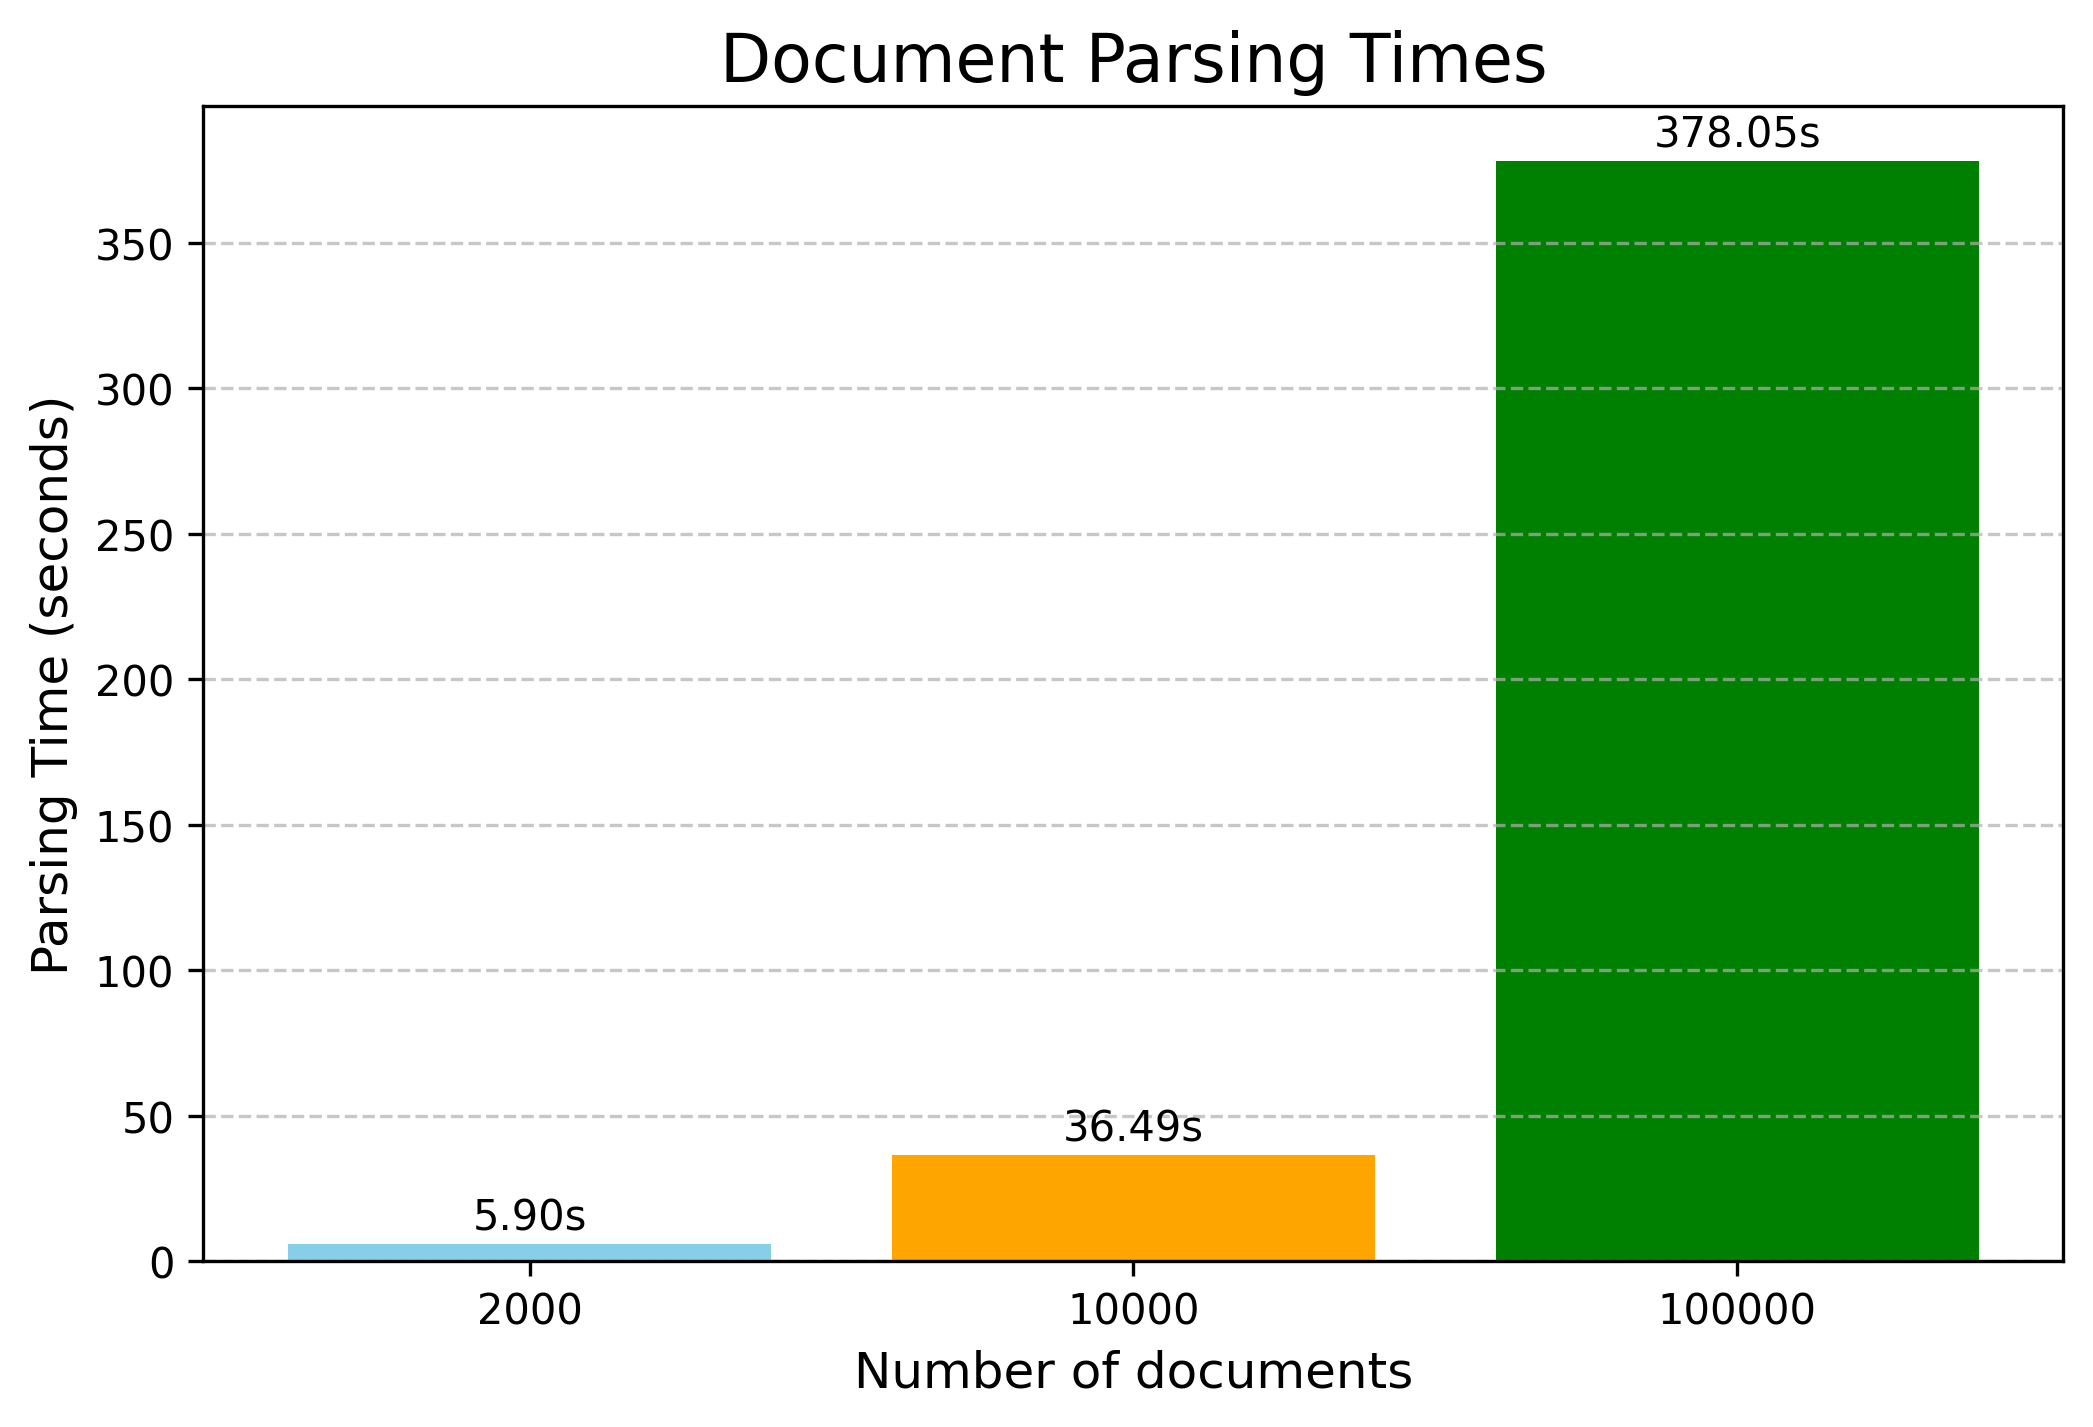
\includegraphics[width=\textwidth]{parsing_times_chart.png}
    \caption{command:'parse'}
    \label{fig:cmd-parse}
\end{figure}
\begin{figure}[h!]
    \centering
    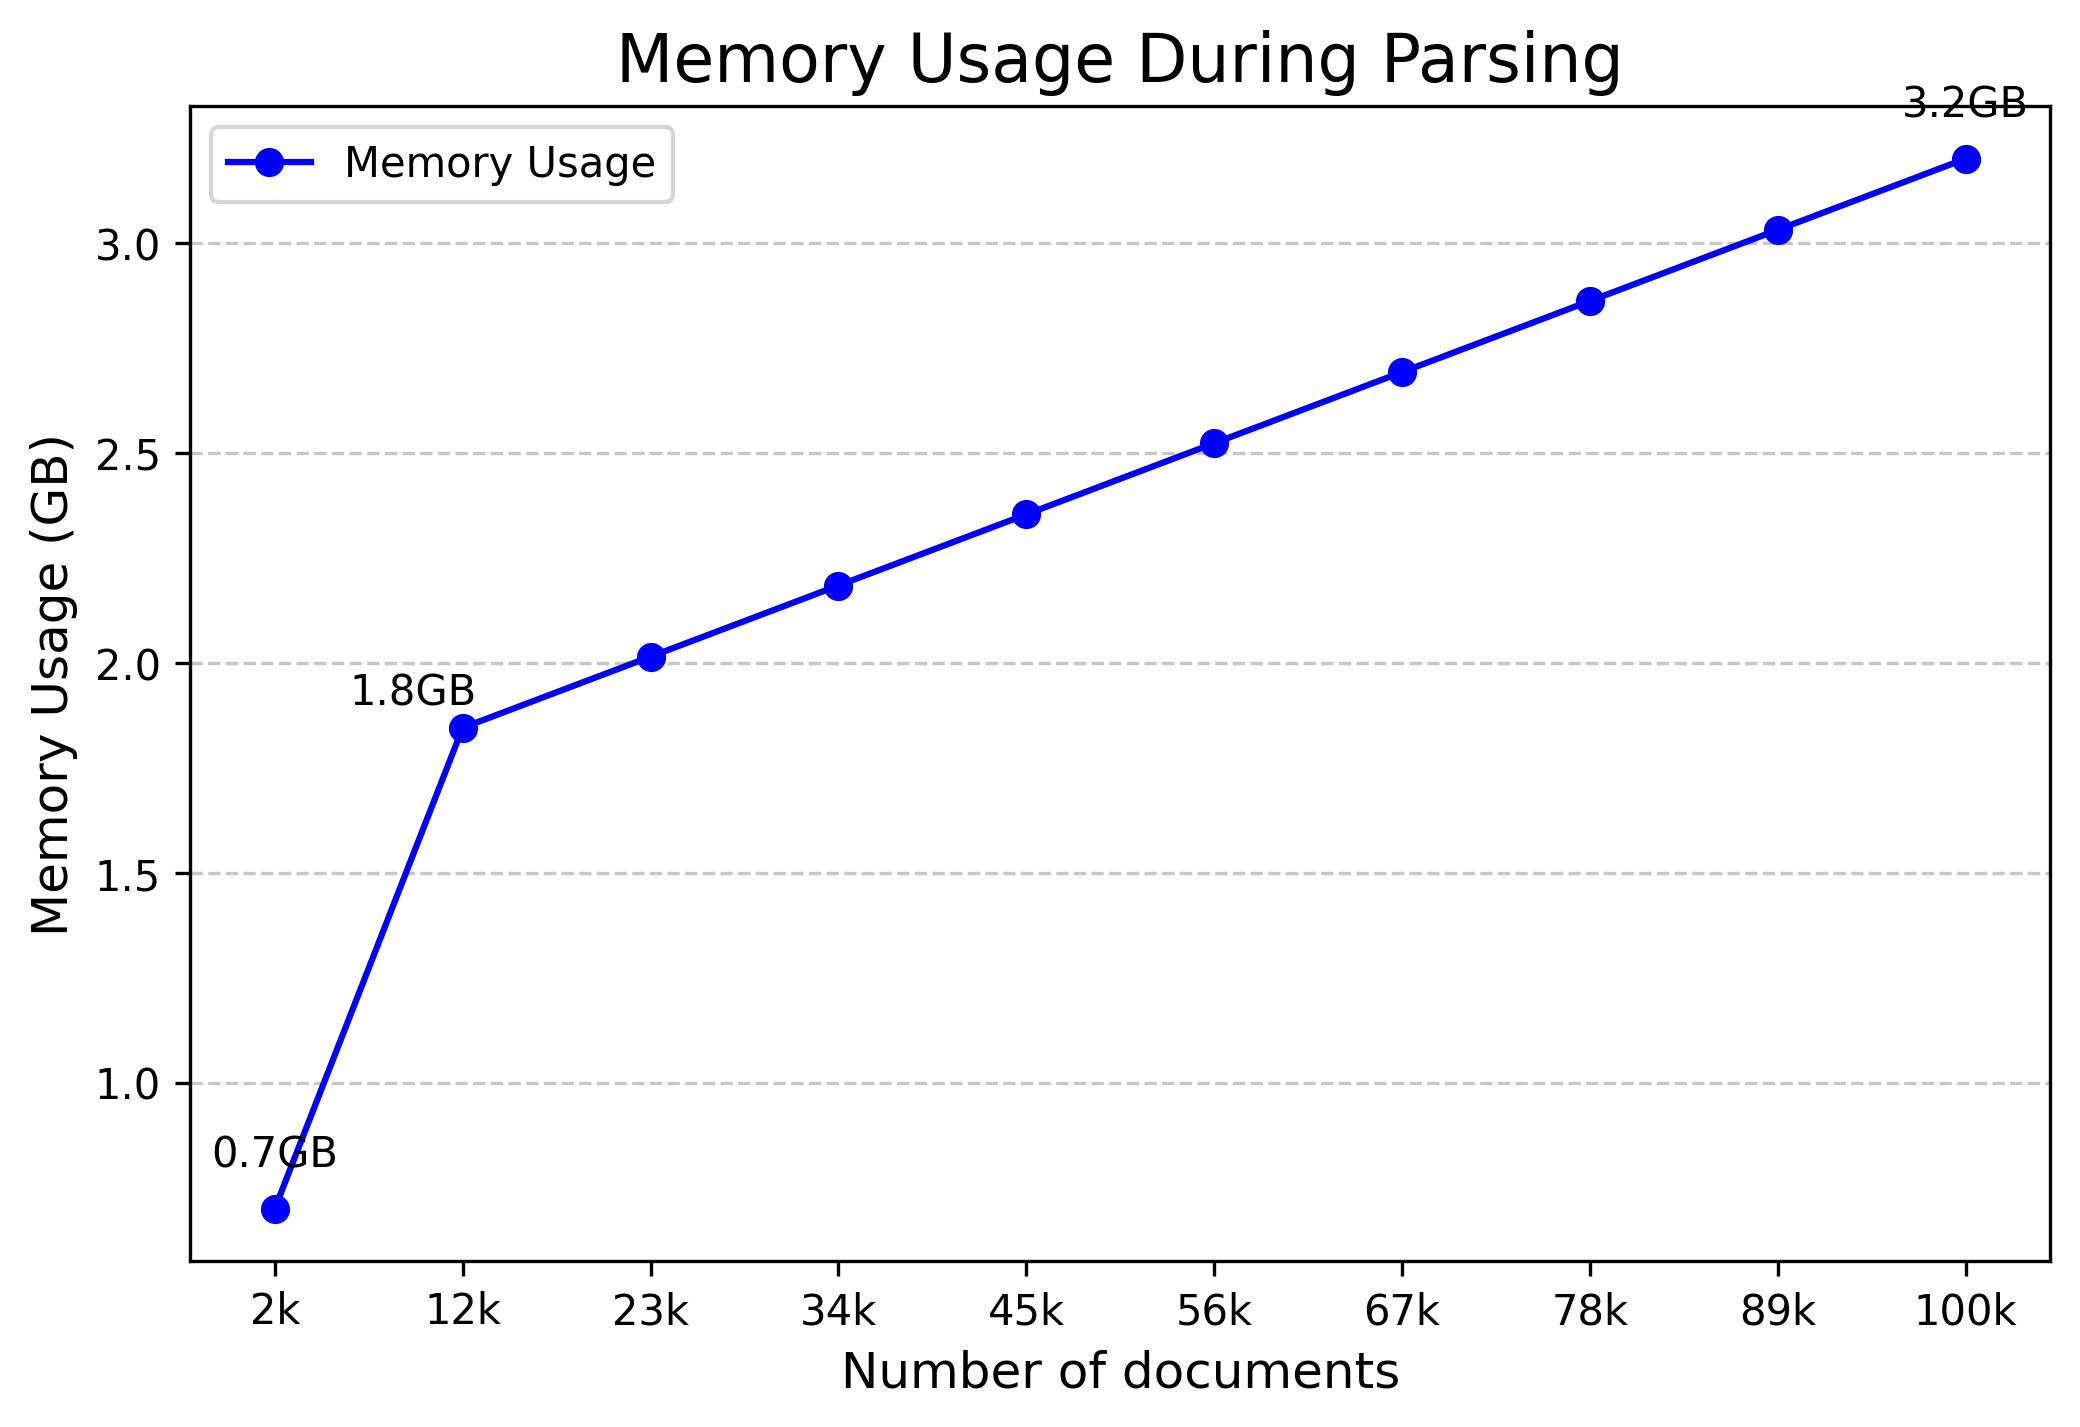
\includegraphics[width=\textwidth]{memory-usage.png}
    \caption{memory usage}
    \label{fig:memory-usage}
\end{figure}

\subsection{Searching}
    \subsection{Initialization}
    To initialize the search engine GoSeek takes less than a second for documents up to 30000 and takes 3 seconds to initialize for 100000 documents. While idle GoSeek uses 1.7GB of memory.
    Figures below  shows correlation between search keywords,memory usage, time it took and number of documents the engine was initialized with for Bitonic Sort and QuickSort algorithms

    \begin{figure}[h!]
        \centering
        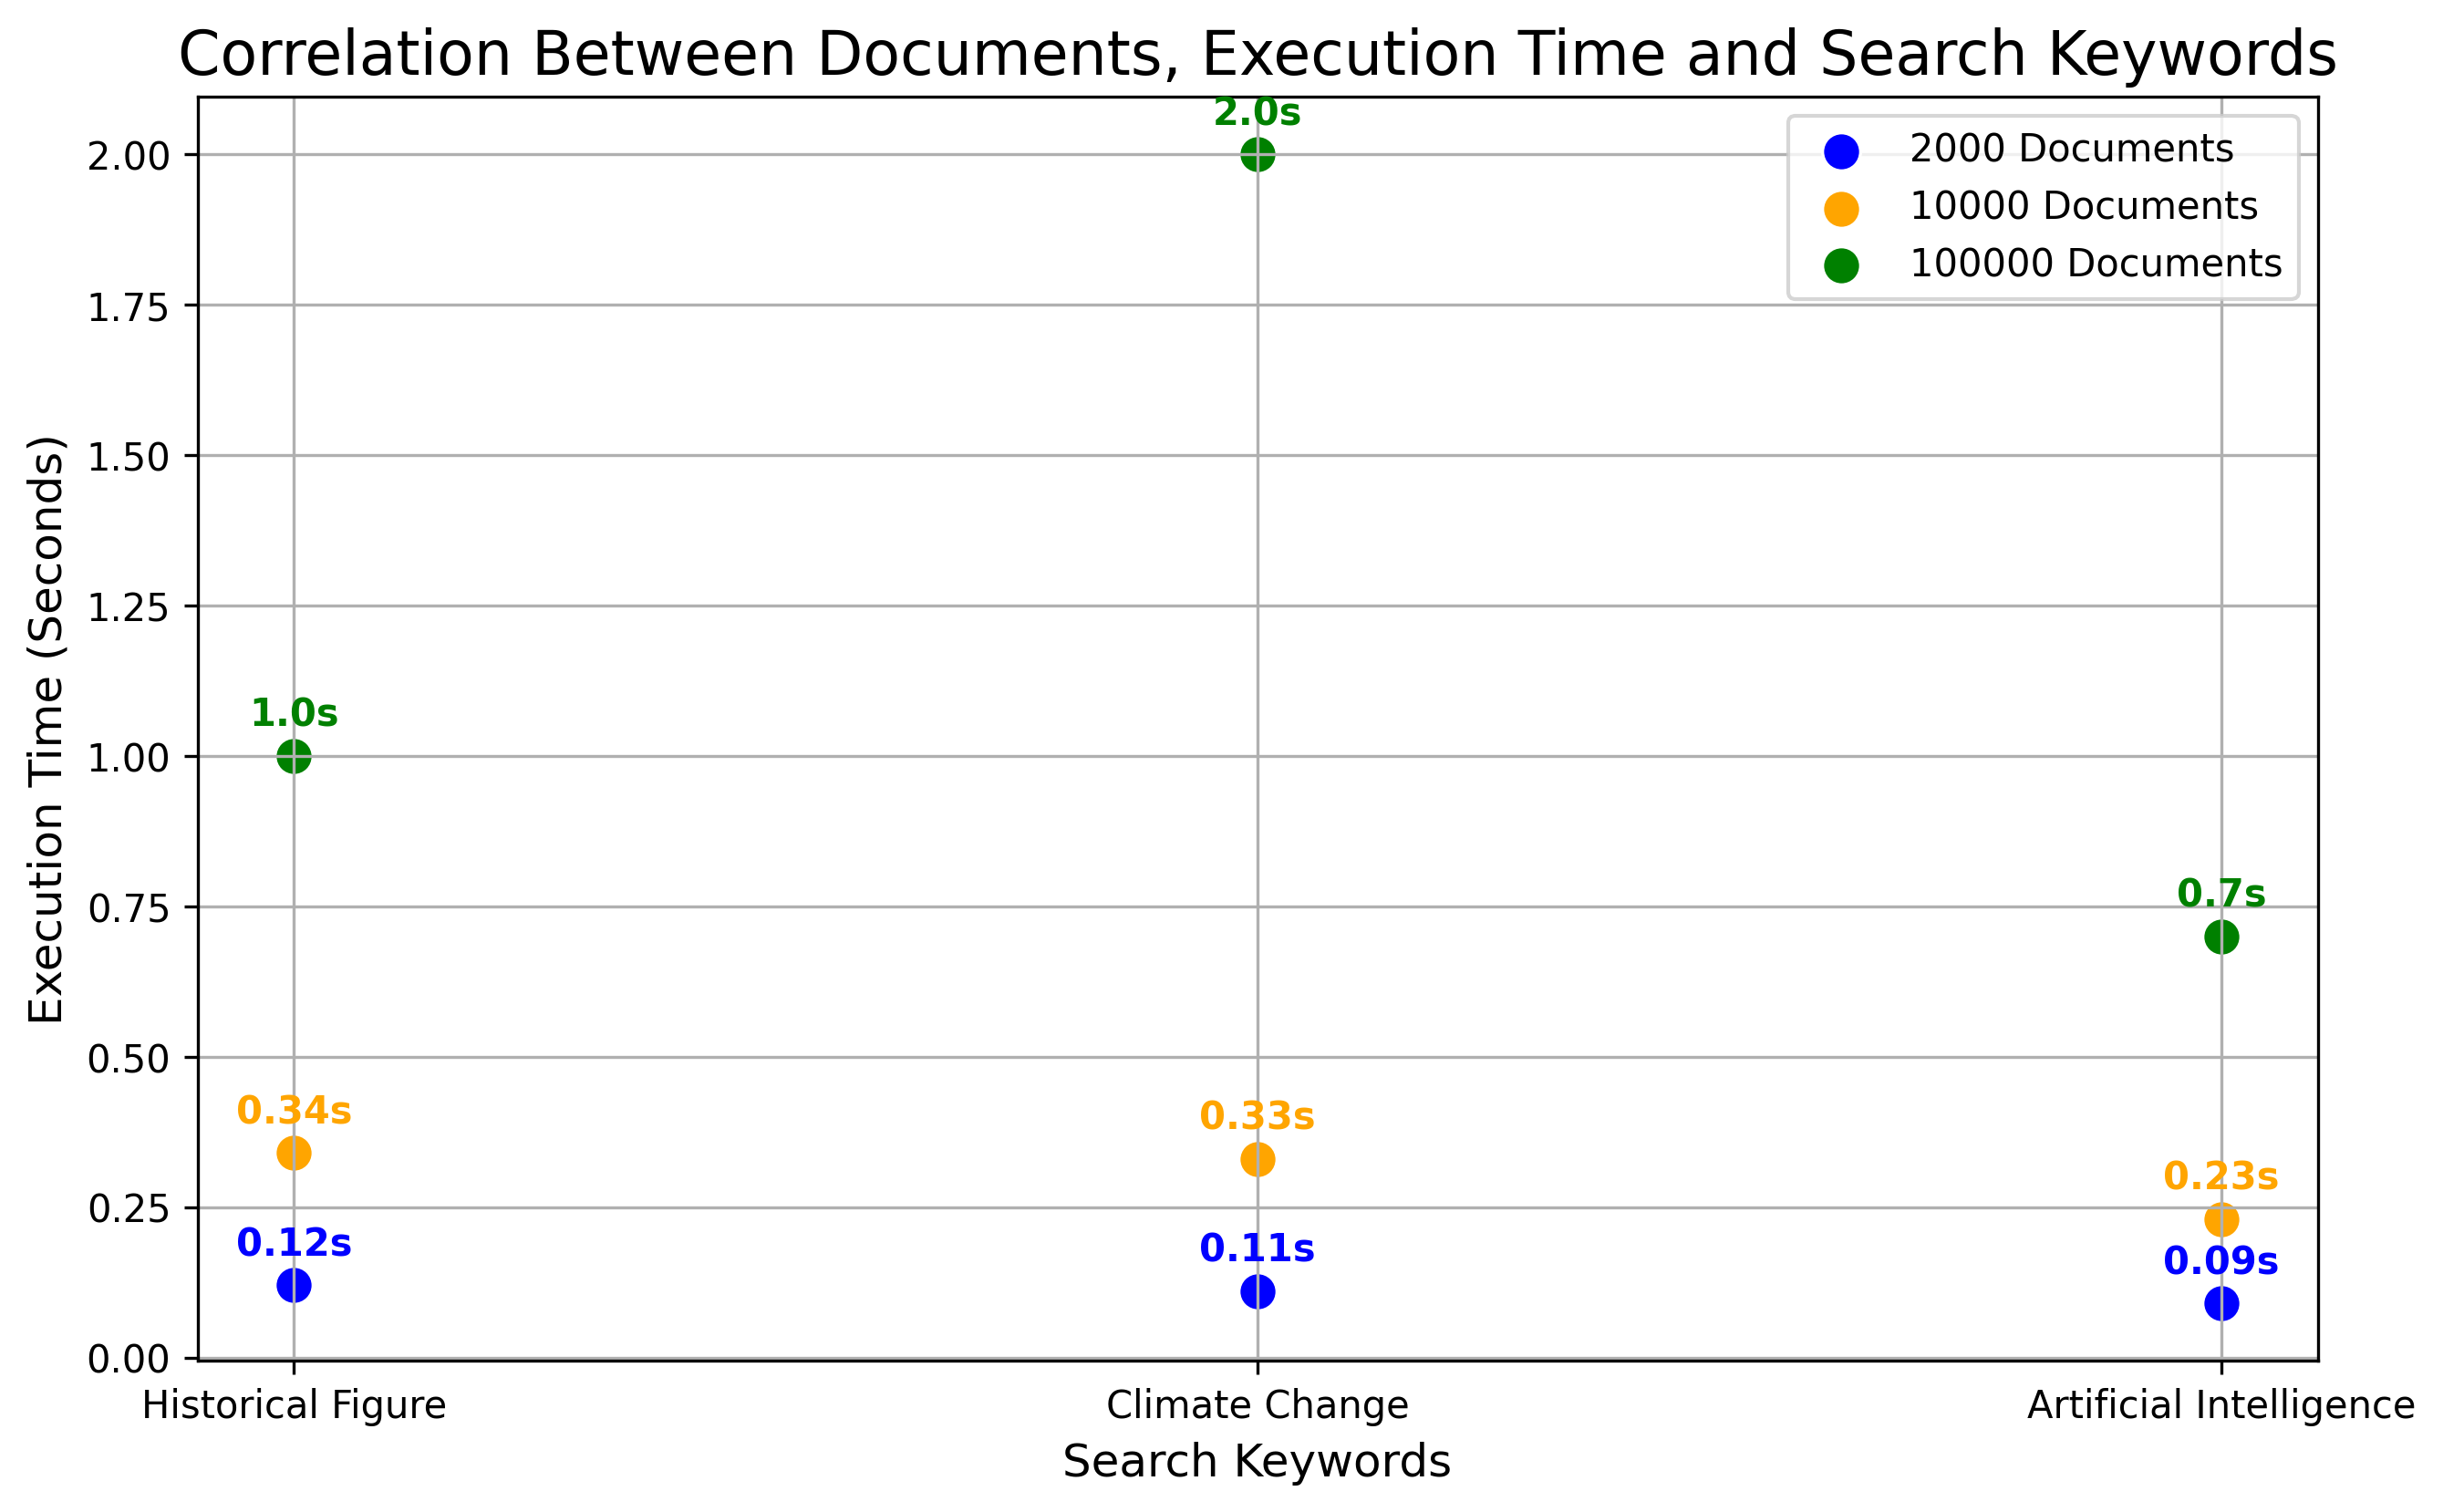
\includegraphics[width=\textwidth]{btsort.png}
        \caption{Bitonic Sort}
        \label{fig:btsort}
    \end{figure}
    \begin{figure}[h!]
        \centering
        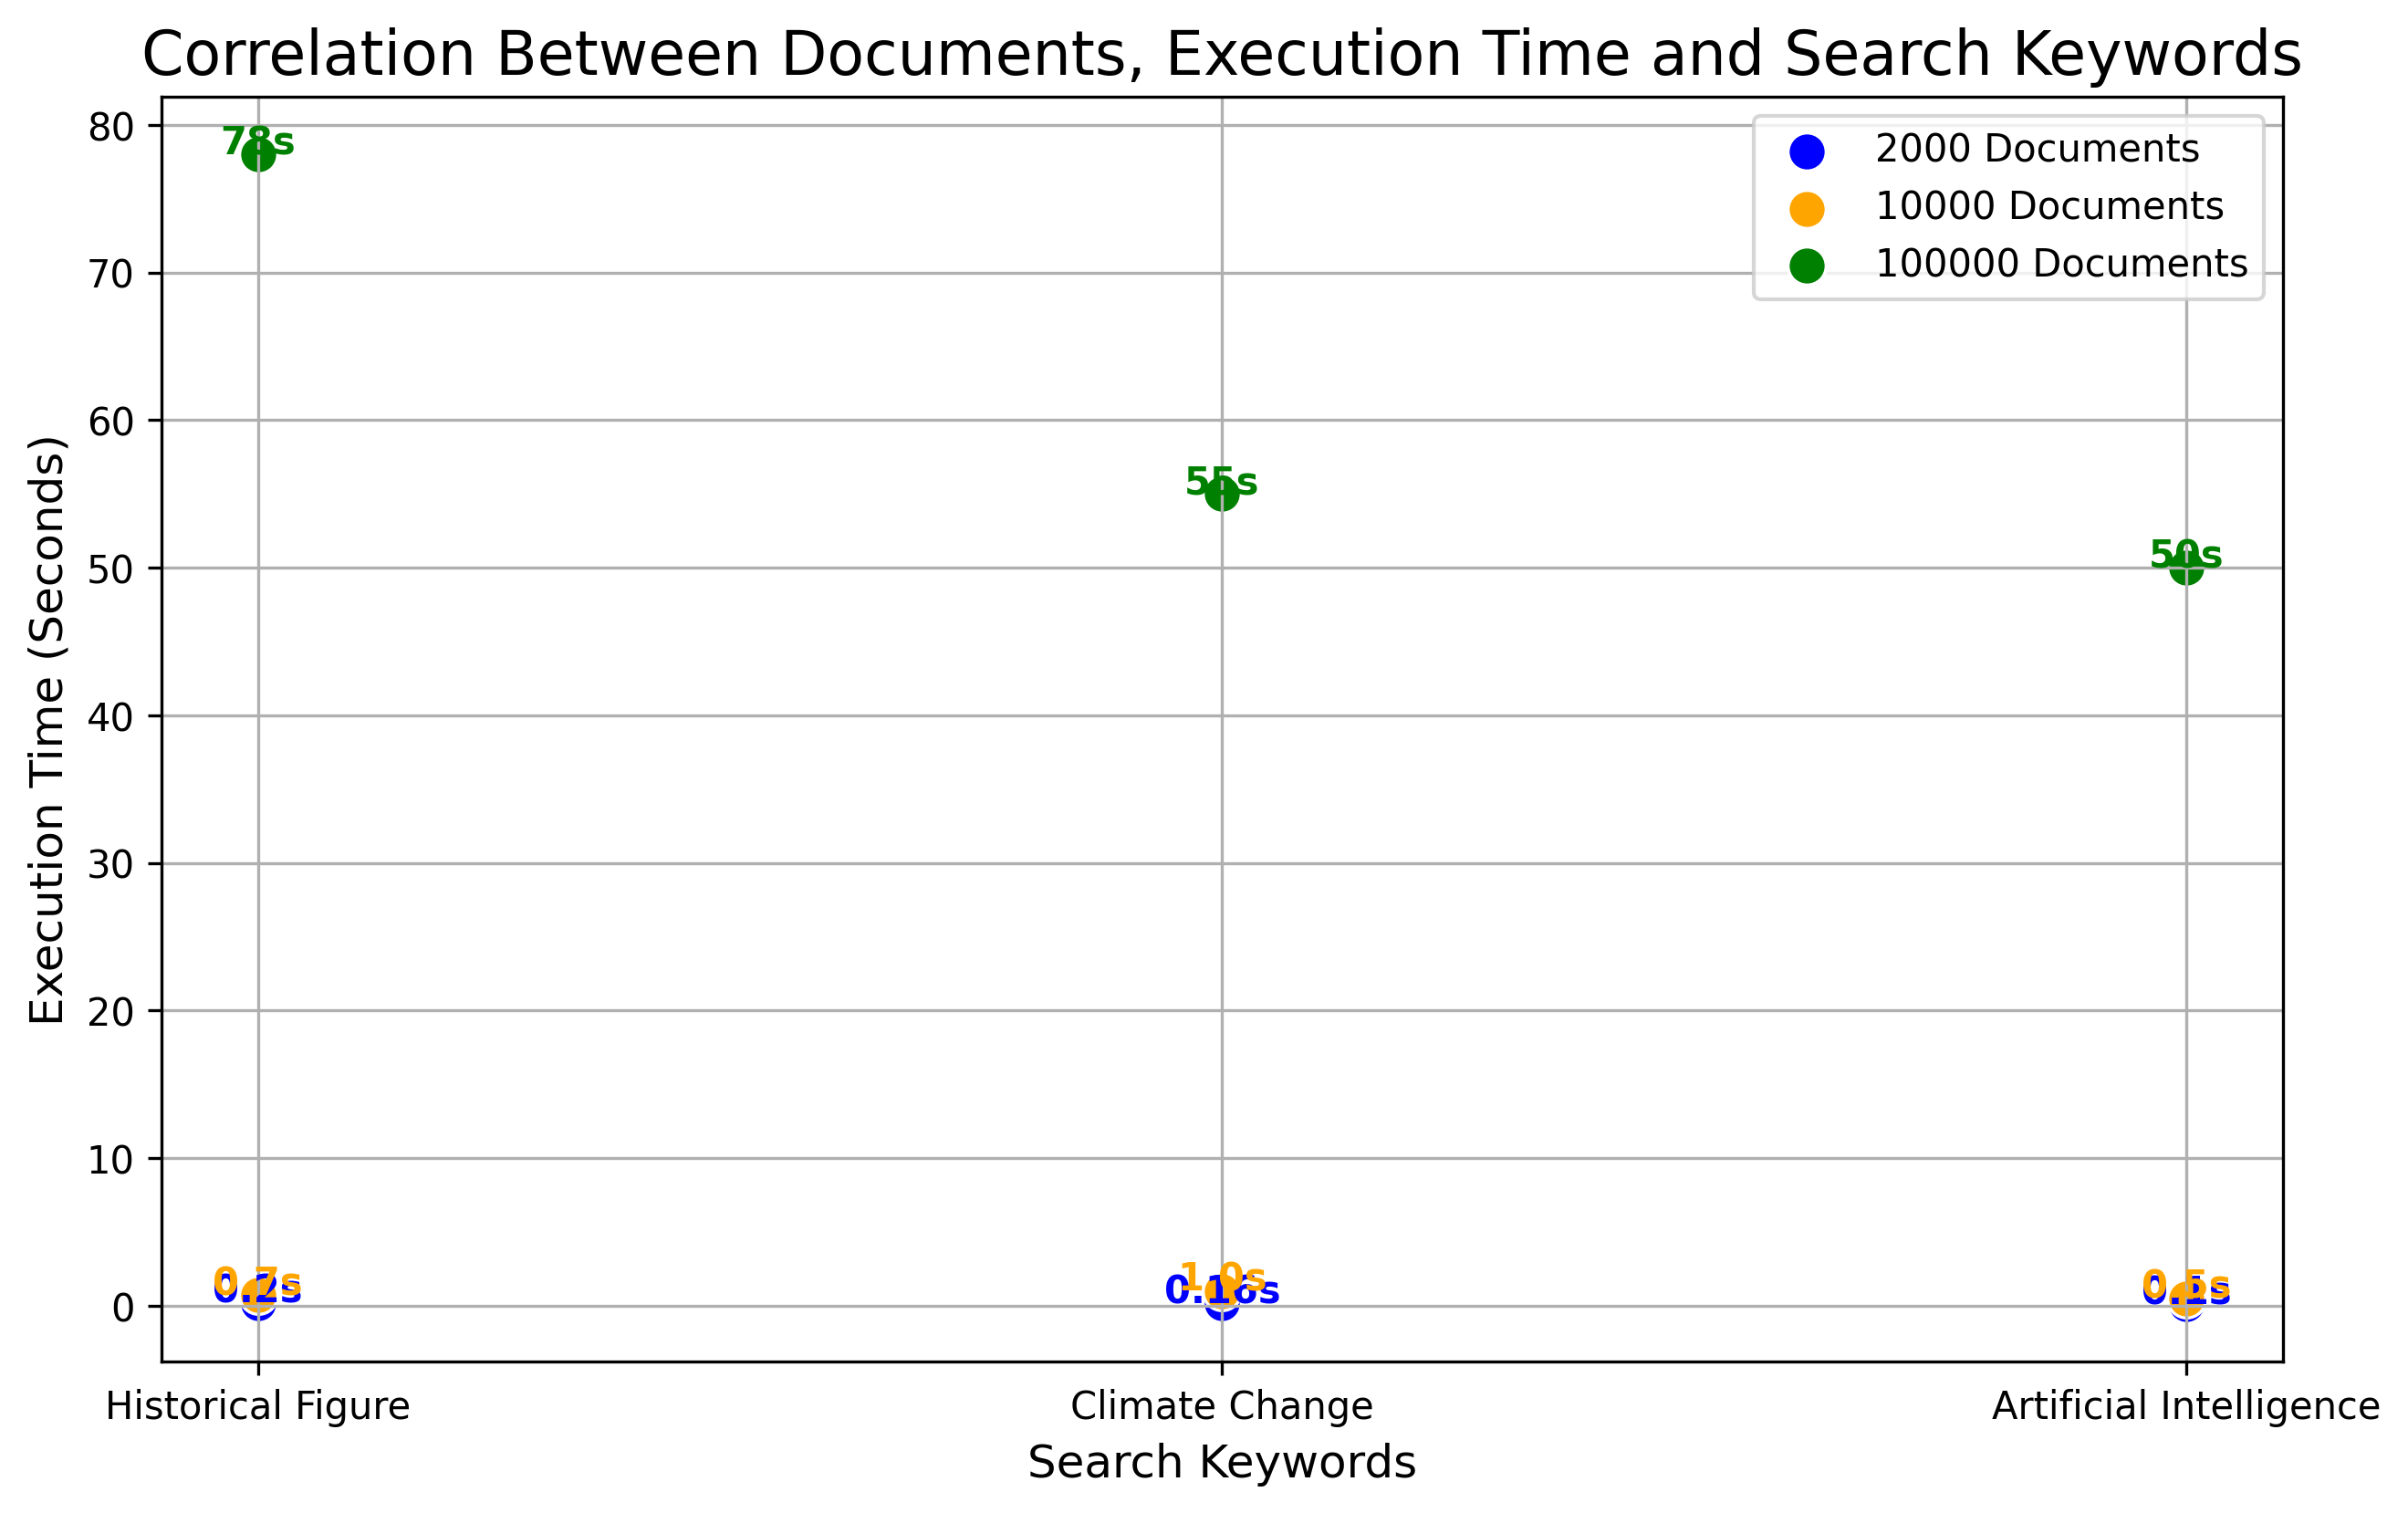
\includegraphics[width=\textwidth]{quicksort.png}
        \caption{Quick-Sort}
        \label{fig:btsort}
    \end{figure}
    \begin{figure}[h!]
        \centering
        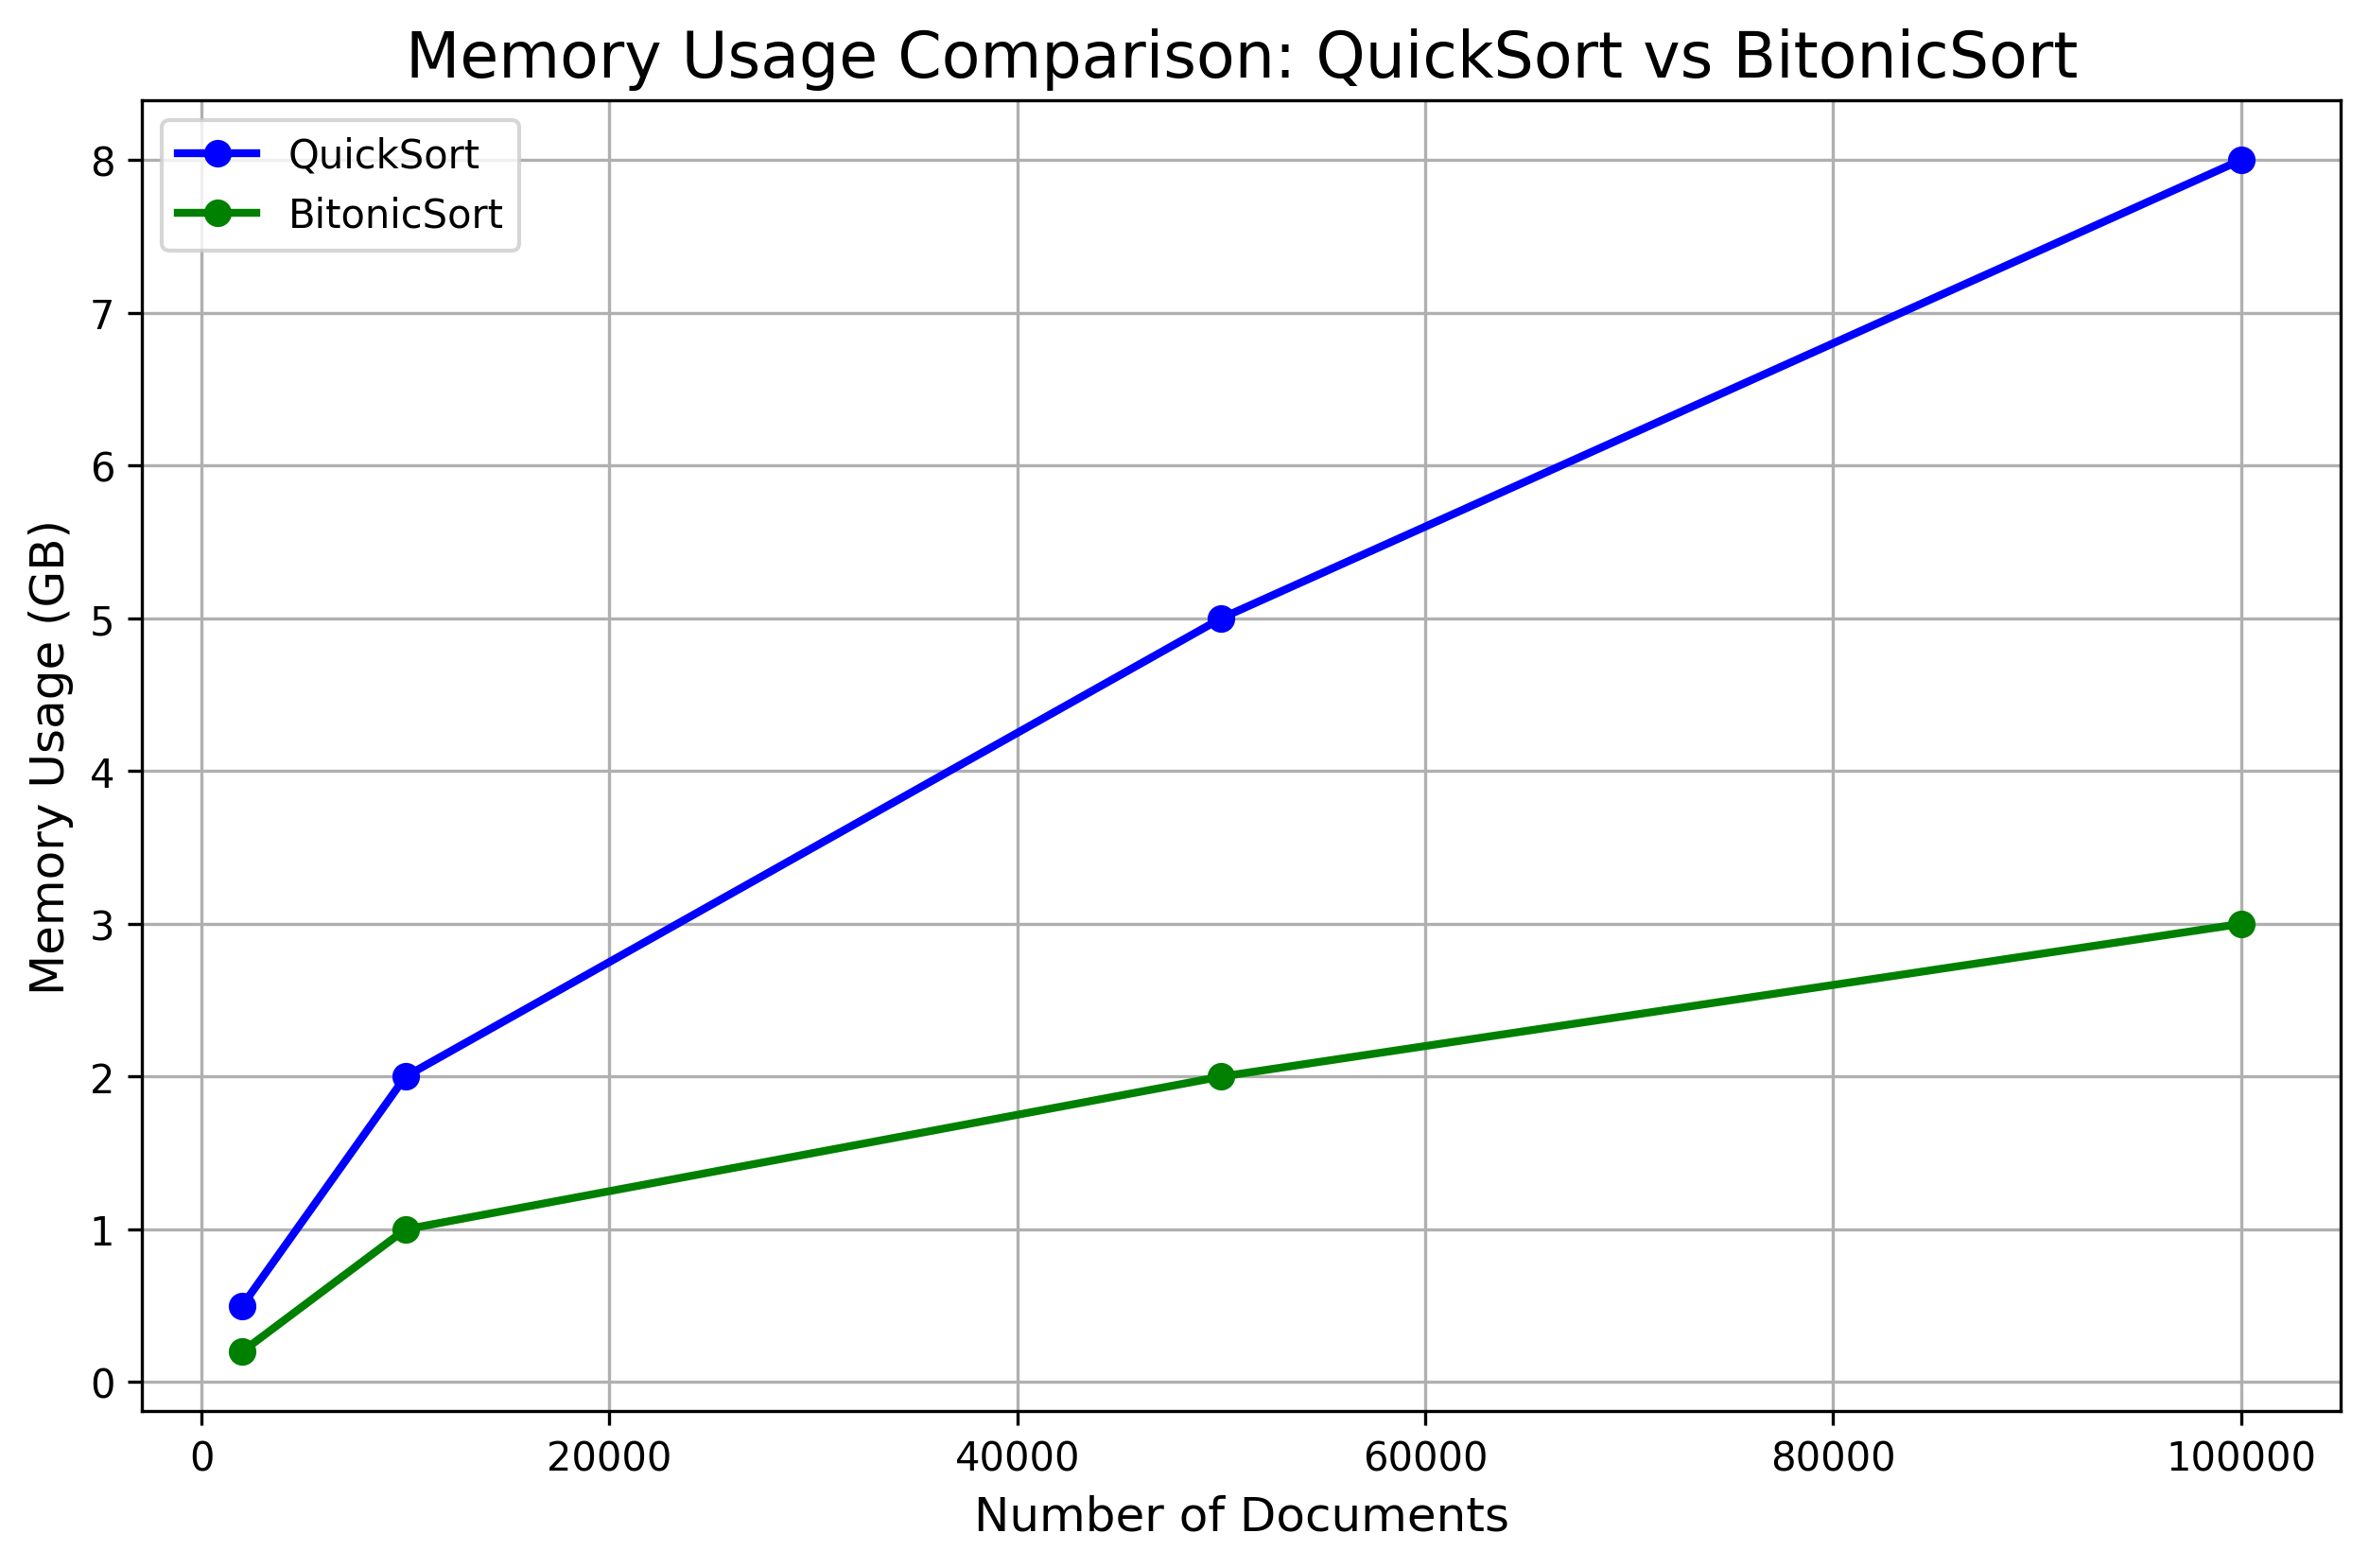
\includegraphics[width=\textwidth]{memory-diff.png}
        \caption{runtime memory usage}
        \label{fig:btsort}
    \end{figure}
    \clearpage
    \subsection{Pattern Matching}
    Pattern matching engine takes less than one second to initialize on all number of documents tested. 
    Figure \ref{fig:pm} below show the correlation between the patterns searched, documents loaded in the engine, and execution time. \\ 
    For more clear understanding of patternMatch capabilities along with the existing \textbf{.json} file , it was tested with 10GB \textbf{.pdf} file. 
    As for memory usage it stays under 800mb.
    \begin{figure}[h!]
        \centering
        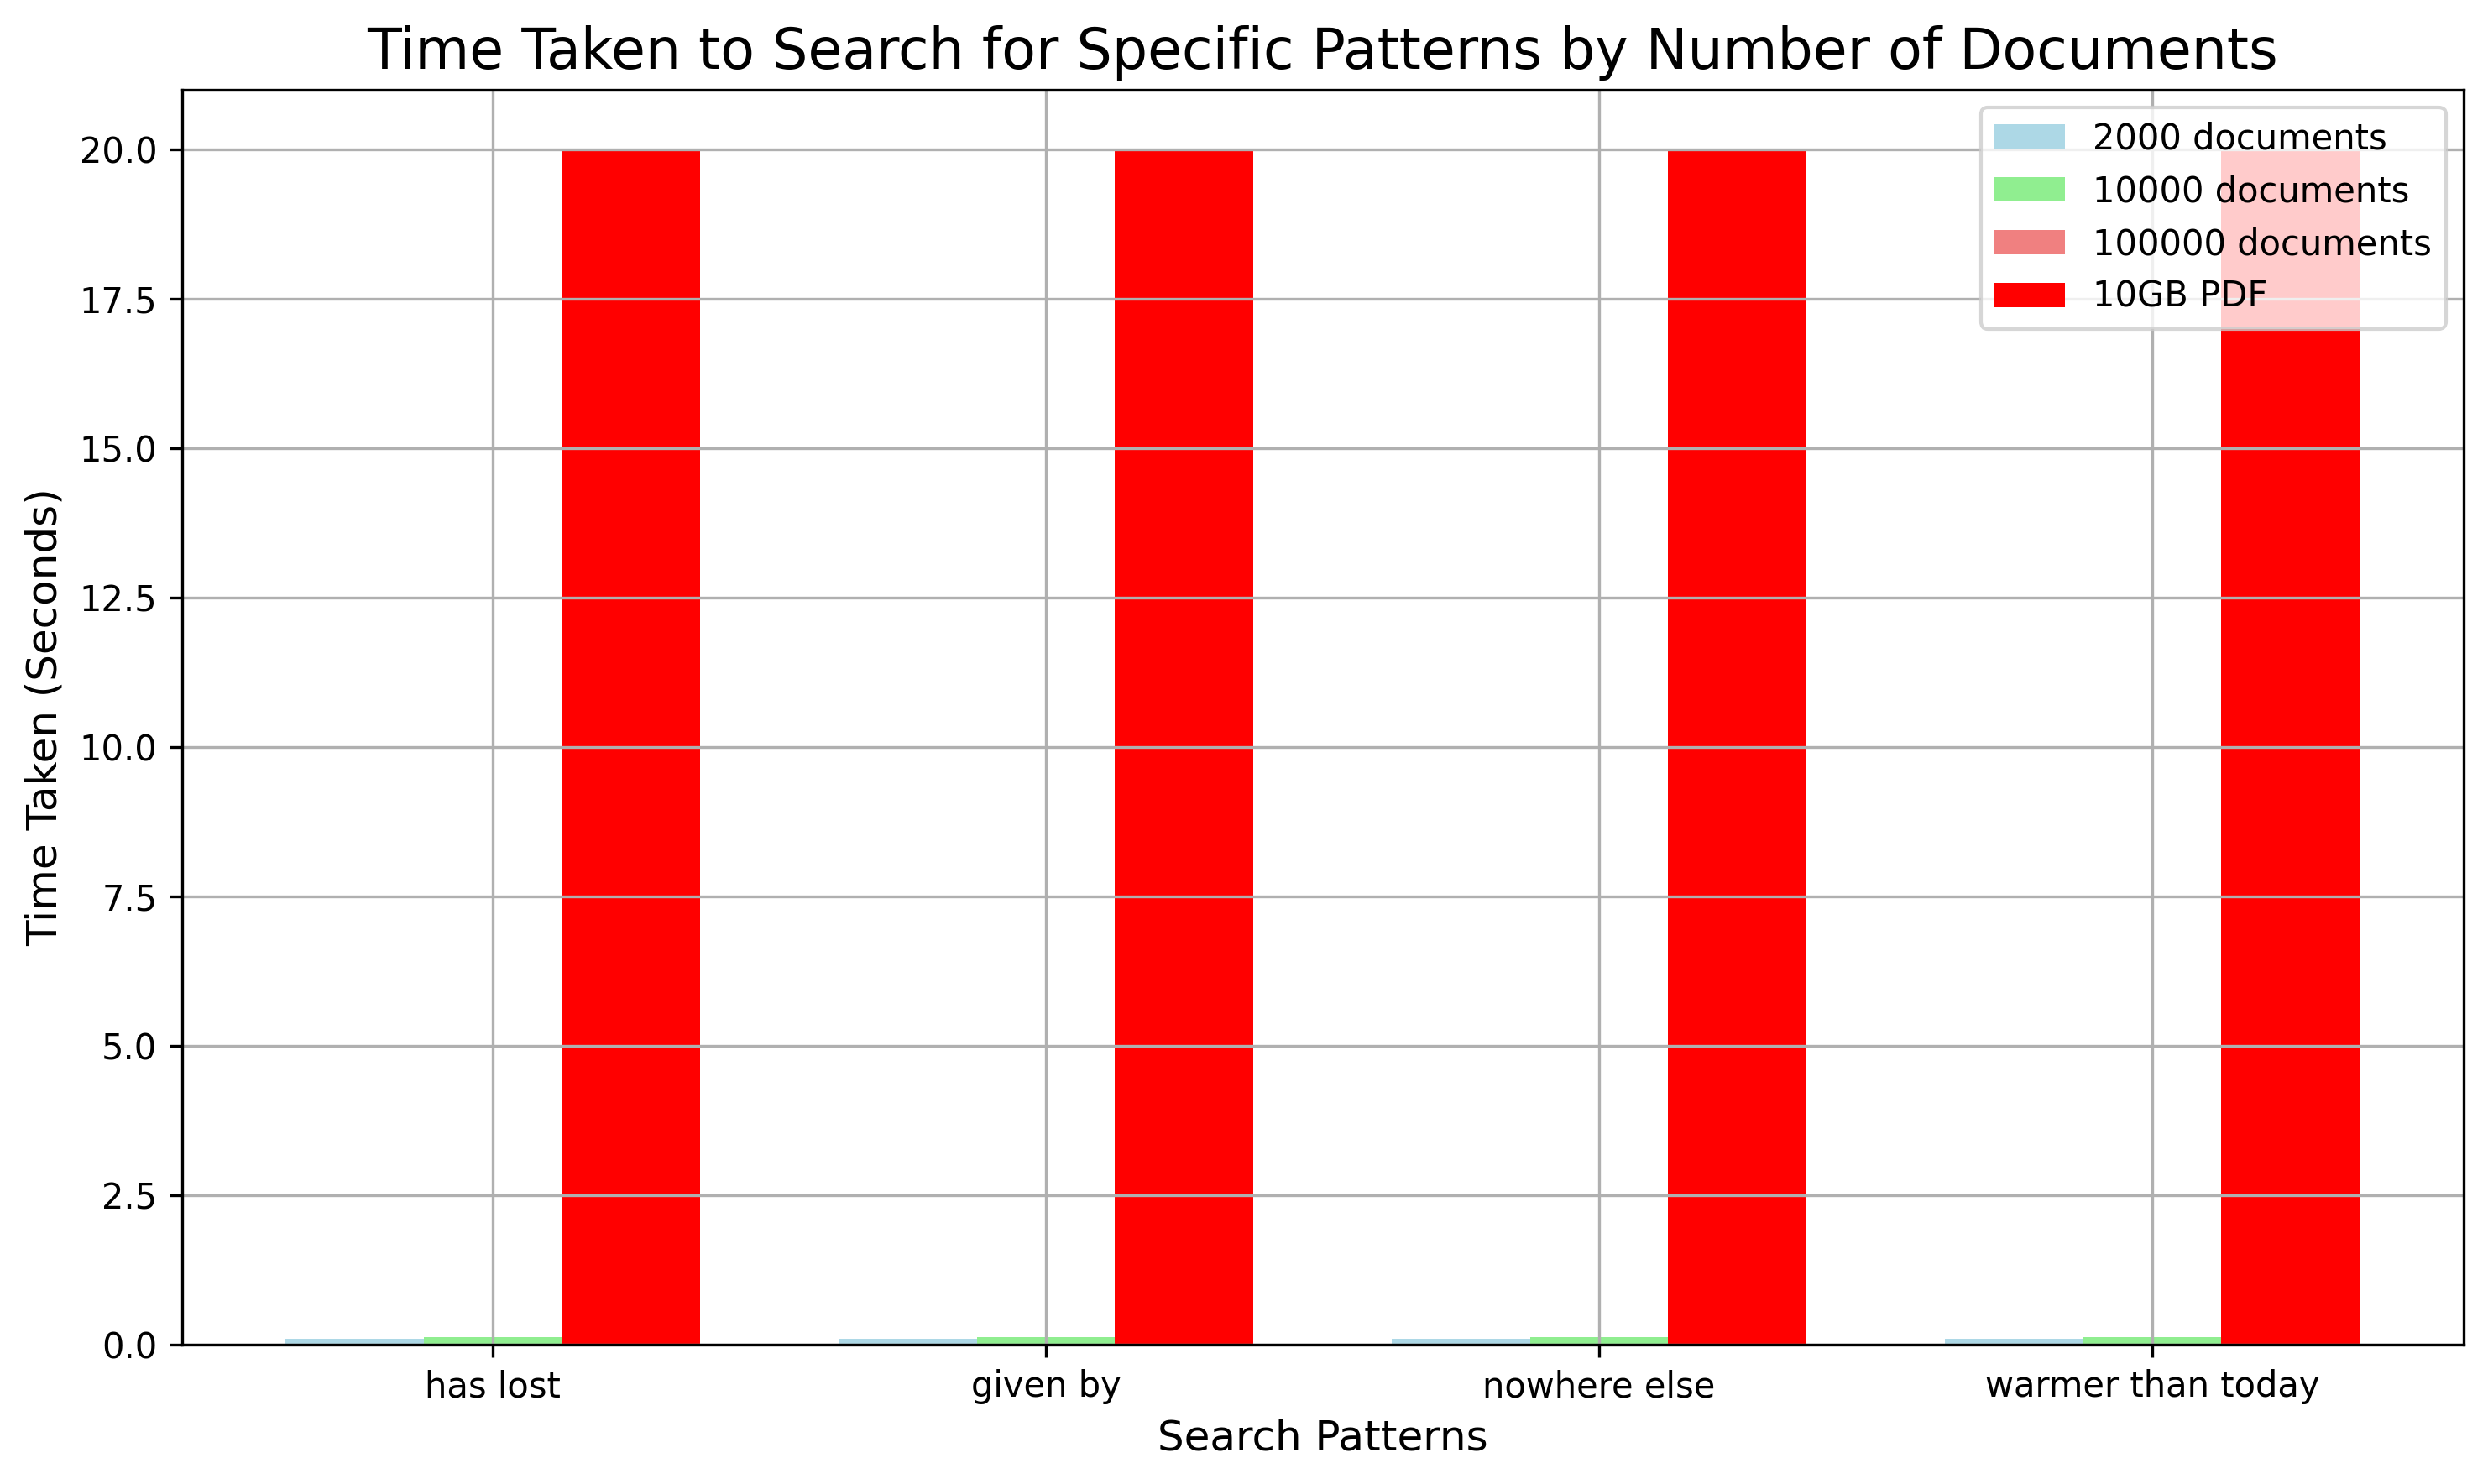
\includegraphics[width=\textwidth]{big-pdf.png}
        \caption{Pattern matching correlations - 300MB input file}
        \label{fig:pm}
    \end{figure}
    \clearpage
\section{Discussion}

The Goseek search engine exhibits outstanding performance and high accuracy when searching for a topic across documents. Its lightweight nature makes it ideal for everyday use by individual users. The tests conducted clearly highlighted the superior performance of the bitonic sort algorithm over other sorting algorithms. Bitonic sort outperformed quicksort by a factor of 76 in terms of speed, while also using significantly less memory. In contrast, quicksort's memory usage increases exponentially as the dataset grows, making it less suitable for large datasets. Additionally, our logs show that bitonic sort does not place a heavy load on CPU usage, operating with fewer than 9,000 concurrent threads, which is easily manageable by modern CPUs. Based on these results, it is safe to conclude that quicksort is not suitable for large datasets. On the other hand, bitonic sort is a scalable and robust solution, even when distributed across multiple machines with the same dataset.

While quicksort is easier to implement and more widely used, it offers no distinct advantages for handling large-scale data. It consumes more memory and is slower in comparison.

The pattern matching engine also demonstrated excellent performance. Searching for a pattern containing three or more words took less than a second in a dataset of 50,000 documents and just 1.2 seconds for 100,000 documents. This demonstrates the efficiency of the Knuth-Morris-Pratt (KMP) algorithm, which processes each character only once. As such, the number of words in the pattern does not significantly impact the execution time. Given this, we can confidently conclude that the KMP algorithm is the ideal choice for all pattern matching applications.

\subsection{Hypothesis Evaluation}

Although we do not have specific comparative data against commercial search engines such as Google or Bing, the results from our implementation show promising potential. Some key highlights include:

\begin{itemize}
    \item Unbiased ranking achieved through the use of Term Frequency-Inverse Document Frequency (TF-IDF)
    \item Advanced pattern matching capabilities
    \item Efficient performance at scale
    \item No advertisement influence on search results
\end{itemize}

\subsection{Strengths}

The Goseek engine possesses several strengths:

\begin{itemize}
    \item Clean, modular architecture adhering to best practices
    \item Comprehensive logging system for performance tracking
    \item Multiple sorting algorithm implementations allowing for performance comparison
    \item Efficient document processing and initialization
    \item Novel combination of TF-IDF with pattern matching
\end{itemize}

\subsection{Weaknesses}

However, there are a few weaknesses:

\begin{itemize}
    \item Limited to a command-line interface
    \item Requires pre-processing of documents before they can be searched
    \item Memory usage could be optimized (1.7GB baseline is significant)
    \item Bitonic sort requires input sizes that are powers of two
\end{itemize}

\subsection{Limitations}

The current work has several limitations:

\begin{itemize}
    \item Testing was conducted on modest hardware (AMD Ryzen 7 3750H, 8GB RAM)
    \item The dataset size used in testing was limited to 100,000 documents
    \item No direct comparison with commercial search engines
    \item The search capability is limited to text in ASCII characters after parsing
\end{itemize}

\subsection{Future Work}
Future work will involve the development of a web interface to make the engine more accessible. By adding a user-friendly interface, Goseek can reach a wider audience, moving beyond its current command-line configuration. \\
Currently GoSeek is great at describing internal processes but analyzing them is up to the user, thus one great addition would be a analyzer command that tells the user \\
all of the performance evaluations based on the already existing logs in a manner which is more readable and accessible to the user.


\clearpage
\chapter{Conclusion}
This thesis effectively demonstrated that building an unbiased search engine using Golang, TF-IDF ranking, and pattern matching is not only feasible but can potentially outperform traditional advertisement-driven search engines in delivering relevant results. Goseek as a command-line tool successfully delivered on its promise of being a lightweight and fast search engine utilizing higher order algorithms.
The integration of bitonic sort proved its superiority to quicksort, showing an improvement in speed by 76 times while maintaining lower memory usage. The pattern matching implementation using the KMP algorithm demonstrated blazingly fast performance and efficiency, processing 100,000 documents in just 1.2 seconds. Perhaps most importantly, the engine maintained consistent performance without compromising accuracy or introducing advertising bias, which was one of the primary motivations for the project.
Looking forward, while Goseek currently exists as a command-line tool with certain limitations, such as its pre-processing of \textbf{.html} documents, despite this, it has established a solid foundation for future development.Its Architecture is robust and easily extandable to any number of file extensions this gives options to other developers to extend its functionality. While there's room for further optimization and feature enhancement,
GoSeek represents a meaningful step toward more transparent and efficient information retrieval systems.










\appendix
\chapter{Appendix}
\begin{itemize}
    \item For more detailed look please the the source code of the project - \\ https://github.com/romanitodua/capstone-project-search-engine
    \item For exploring the logs more in detail please see the \textbf{/logs} directory of the source code
    \item For developer build please see the \textbf{dev} branch of the source code
\end{itemize}

% References
\printbibliography[heading=bibintoc] 
\end{document}
